% Chapter 2

\chapter{Requisite Mathematics} % Main chapter title
\label{ch:math} % For referencing the chapter elsewhere, use \ref{Chapter1} 

\lhead{Chapter 2. \emph{Requisite Mathematics}} % This is for the header on each page - perhaps a shortened title

%----------------------------------------------------------------------------------------

This chapter presents some of the basic math involved in constructing and training Deep Learning models. The concepts presented in this chapter assume few results from Linear Algebra and Probability Theory.  Further, we will consider the numerical computation issues that come into play while implementing the theory in practice. an attempt to develop some intuition about the high-dimensional statistics involved in the trained models is presented in the last section.

\section{Backpropogation and Automatic Differentiation}
\label{sec:bpad}
The invention of the backpropagation algorithm was the turning point in the history of Neural Networks. It allowed efficient computation of the gradients of the cost function with respect to all the parameters in the model. For any \textit{unrolled} set of parameters. We need to calculate the partial derivatives of the cost $J$ with respect to each $\theta _{i} \in \bm{\theta}$. The function J is given by,
\begin{equation}
J(\bm{x},\bm{\hat{y}};\bm{\theta}) = L(f(\bm{x};\bm{\theta}), \bm{\hat{y}})
\end{equation}
Therefore, the gradients we need to determine are:
\begin{equation}
\nabla _{\bm{\theta }} J \frac{\partial J }{\partial \bm{ \theta }}
\end{equation}

The choice of the loss function $L$ is elaborated in the next section.

Automatic Differentiation can be viewed as the generalised version of backpropagation. The fundamental concept is the application of chain rule at the operator level, for the evaluation of the gradient. We setup a computational graph as a composition of primitive operations. Every node takes multiple variables as arguments and has outputs. The chain rule states that the gradient with resepct to the output can be split in terms of the input.

Ex.
\begin{align*}
L &= x + y			&		L &= x * y \\
\frac{\partial L}{\partial x} &= 1 & \frac{\partial L}{\partial x} &= y\\
\frac{\partial L}{\partial y} &= 1 & \frac{\partial L}{\partial y} &= x
\end{align*}

\section{Loss Functions}

Loss functions determine the error that backpropagates through the network. It quantifies the error produced by the network on a training sample with reagrd to the labeled target value.

\subsection*{Euclidean Distance / Mean-Squared Error (MSE)}
The plain vanilla Euclidean distance of the $L^2$ norm can be used to measure the error between output vectors. Use of this function is not practical in large networks as the gradient explodes due the quadratic nature of the curve.
\begin{equation}
J(\hat{\bm{y}},f(\bm{x};\bm{\theta})) = ||\hat{\bm{y}} - f(\bm{x};\bm{\theta})||^{2}
\end{equation}
where $f(\bm{x};\bm{\theta})$ is the output from the model and $\bm{y}$ is the labeled target for the training example.





\subsection*{Cross-Entropy Loss}
When we have two separate probability distributions $P(\bm{x})$, $Q(\bm{x})$ defined over the same random variable $\bm{x}$, we can define the \textit{divergence} of the pair of distributions. It is a measure of how dissimilar the two probability distributions are. Information theory provides a useful method of measuring this divergence called \textit{Kullback-Leibler (KL) divergence}:
\begin{equation}
\label{eq:celoss}
D_{KL}(P \parallel Q) = E_{x \sim P}\left[log \frac{P(\bm{x})}{Q(\bm{x})}\right]
\end{equation}
Some immediate properties that become evident from this equation are that the value of $D_{KL}(P\parallel Q) = 0$ only if $P(\bm{x})$ and $Q(\bm{x})$ are the same probability distribution. Further, the divergence measured is always non-negative and can be interpreted as a type of distance metric, much like Euclidean distance. Notice however that $D_{KL}(P \parallel Q) \neq D_{KL}(Q \parallel P)$. Therefore KL divergence is not a symmetric operation. This brings us to our definition of \textit{cross-entropy loss},
\begin{equation}
H(P,Q) = H(P) + D_{KL}(P \parallel Q)
\end{equation}
From Eq.\ref{eq:celoss}, it can be seen that this is equivalent to,
\begin{equation}
H(P,Q) = -E_{x \sim P}\left[ \log Q(\bm{x})\right]
\end{equation}
Therefore, minimizing the cross-entropy loss is w.r.t. $Q$ is equivalent to minimizing the KL divergence. This makes sense intuitively since we want the distribution of the laebelled target value $\hat{\bm{y}}$ to match the output of the model $f( \bm{x} ; \bm{ \theta } )$ Also, the output allows for a probabilistic interpretation of the output vector.
\section{Activation Functions}
Activation Functions are in a sense the essence of the functionality of Neural Networks, they introduce the non-linearities that allow the network to learn the complex decision boundaries in high dimension space (discussed in sec.\ref{sec:highds}) Our choice of activation ffunction is guided by the following considerations:
\begin{itemize} \itemsep -3pt
\item Saturation of function for high input value i.e. vanishing gradient.
\item Centering of values around zero for even distribution of activations.
\end{itemize}
We evaluate the following functions based on these two considerations along with explanations for the requirements.

\subsection*{Sigmoid}
 The sigmoid function $\sigma(\bm{x})$ is defined as $\sigma(\bm{x}) = 1/1+e^{-\bm{x}}$. This activation was traditionally the de facto non-linearity added to hidden layers as it resembled the firing of a biological neuron i.e. \textit{zero} being inactive and \textit{one} being active/firing. THe sigmoid function had worked relatively well for training neural networks for a long time, but posed an important issue for the larger models. several coumpounded activations over multiple layers led to the \textit{saturation} of the neuron. This means that the value of the function at $\mod 3 $ is at $0.95$. As you can notice, the gradient of the graph also tends to zero beyond these points. We require the gradient to be non-zero for all segments of the firing of the neuron, as the error information back propagates through all layers via the activation value as explained in sec.\ref{sec:bpad}. \\

\begin{figure}[H]
	\centering
	\begin{tikzpicture}

	\datavisualization [scientific axes=clean,
                    visualize as smooth line,
                    y axis={label={$y= \sigma (x)$}},
                    x axis={label} ]

	data [format=function] {
      var x : interval [-6:6] samples 100;
      func y = 1 / (1 + exp( -1 * \value x ));
      };
	\end{tikzpicture}
\caption{Sigmoid activation function}
\label{fig:sigm}
\end{figure}

The sigmoid function was popular due to the convenience of representing its gradient in terms of itself, i.e.
\begin{align*}
\sigma(x) &= \frac{1}{1 + e^{-x}}\\
\frac{\partial \sigma }{\partial x} &= \frac{e^{-x}}{1+e^{-x}} = (\sigma (x)\left(1-\sigma (x)\right)\\
\end{align*}

\subsection*{Hyperbolic Tangent}

\begin{figure}[H]
	\centering
	\begin{tikzpicture}
	\datavisualization [scientific axes=clean,
                    visualize as smooth line,
                    y axis={label={$y=tanh(x)$}},
                    x axis={label} ]

	data [format=function] {
      var x : interval [-4:4] samples 100;
      func y = (1 - exp( -2 * \value x))/(1 + exp( -2 * \value x));
      };
	\end{tikzpicture}
\caption{Hyperbolic tangent activation fnction}
\label{fig:tanh}
\end{figure}
\begin{align*}
tanh(x) &= \frac{1 - e^{-2x}}{1 + e^{-2x}}\\
\frac{\partial tanh(x) }{\partial x} &= 1 - tanh(x)^2
\end{align*}
\begin{figure}[H]
	\centering
	\begin{tikzpicture}
	\datavisualization [scientific axes=clean,
                    visualize as smooth line,
                    y axis={label={$y=max( -1, min( 1, x))$}},
                    x axis={label} ]

	data [format=function] {
      var x : interval [-4:4] samples 100;
      func y = max( -1, min( 1, \value x));
      };
	\end{tikzpicture}
\caption{Hard Hyperbolic tangent activation fnction}
\label{fig:tanh}
\end{figure}

\subsection*{Rectified Lineinar Unit (ReLU)}

\begin{figure}[H]
	\centering
	\begin{tikzpicture}
	\datavisualization [scientific axes=clean,
                    visualize as smooth line,
                    y axis={label={$y=max(0,x)$}},
                    x axis={label} ]

	data [format=function] {
      var x : interval [-4:4] samples 100;
      func y = max( 0, \value x);
      };
	\end{tikzpicture}
\caption{ReLU activation function}
\label{fig:relu}
\end{figure}

\begin{align*}
 o(x) &= max(0,x)\\
\frac{\partial o(x) }{\partial x} &= 1, x > 0 & 0, x \le 0
\end{align*}

\begin{figure}[H]
	\centering
	\begin{tikzpicture}
	\datavisualization [scientific axes=clean,
                    visualize as smooth line,
                    y axis={label={$y=max(\alpha x,x)$}},
                    x axis={label={$x, \alpha = 0.1$}} ]

	data [format=function] {
      var x : interval [-4:4] samples 100;
      func y = max( 0.1 * \value x, \value x);
      };
	\end{tikzpicture}
\caption{Leaky ReLU activation function}
\label{fig:lrelu}
\end{figure}



\subsection*{Softplus}

\begin{figure}[H]
	\centering
	\begin{tikzpicture}

	\datavisualization [scientific axes=clean,
                    visualize as smooth line,
                    y axis={label={$y= \zeta (x)$}},
                    x axis={label} ]

	data [format=function] {
      var x : interval [-6:6] samples 100;
      func y = ln(1 + exp( \value x ));
      };
	\end{tikzpicture}
\caption{softplus activation function}
\label{fig:sigm}
\end{figure}

\section{Optimisation}

\begin{figure}[H]
	\centering
	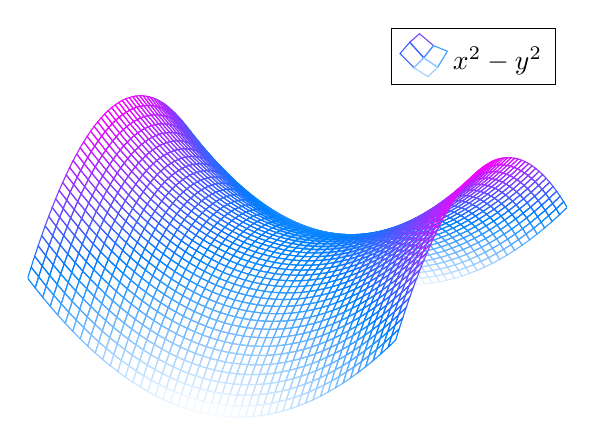
\begin{tikzpicture}
	\begin{axis}[
	    hide axis,
	    colormap/cool,
	]
	\addplot3[
	    mesh,
	    samples=50,
	    domain=-8:8,
	]
	{(x^2-y^2)};
	\addlegendentry{$x^2 - y^2$}
	\end{axis}
	\end{tikzpicture}
\caption{Saddle Point}
\label{fig:sadp}
\end{figure}

\begin{figure}[H]
	\centering
	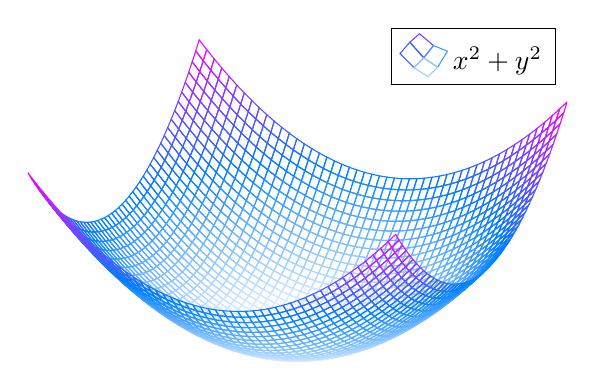
\begin{tikzpicture}
	\begin{axis}[
	    hide axis,
	    colormap/cool,
	]
	\addplot3[
	    mesh,
	    samples=50,
	    domain=-8:8,
	]
	{(x^2+y^2)};
	\addlegendentry{$x^2 + y^2$}
	\end{axis}
	\end{tikzpicture}
\caption{Minima}
\label{fig:minp}
\end{figure}

\subsection*{Stochastic Gradient Descent and its variants}
Stochastic Gradient Descent is the de facto method for training any Neural Network. The basic equation for the parameter updates using SGD is give by,
\begin{equation}
\theta_ i := \theta_i - \alpha \frac{\partial J}{\partial \theta_i}
\end{equation}
\subsection*{Comparison}

\begin{figure}[H]
	\centering
	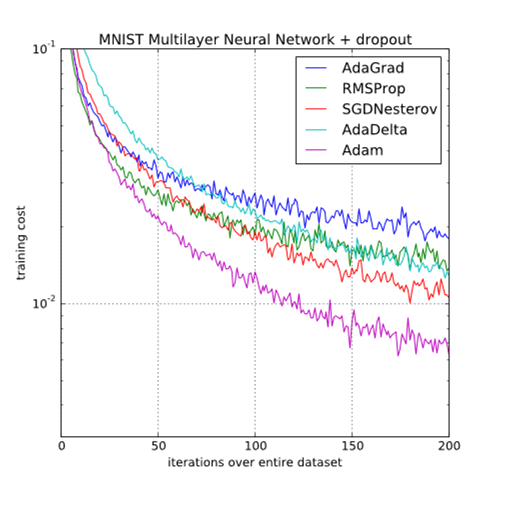
\includegraphics[scale=0.4]{Pictures/convergrate.png}
	\rule{35em}{0.5pt}
	\caption[gd]{Convergence rates of various Gradient Descent algorithms.}
	\label{fig:converg}
\end{figure}




